\documentclass[11pt]{beamer}
\usetheme{default}
\usepackage[ascii]{inputenc}
\usepackage[T1]{fontenc}
\usepackage{amsmath}
\usepackage{amsfonts}
\usepackage{amssymb}
\usepackage{graphicx}
\begin{document}
\begin{center}

\includegraphics[width=11cm,height=8cm,clip]{TitlePageMCS2019.png}
\end{center}
\author{Engr Celso Bation Co, Ph.D, PECE}
\title{Switch Mode Power Supply (SMP) Electronics: An Alternative Perspective}
\subtitle{}
\logo{
\includegraphics[width=.15\linewidth,height=.4cm]{LogoNTS2019.png}}
\institute{Technological Institute of the Philippines}
\date{}
\subject{}
\setbeamercovered{transparent}
\setbeamertemplate{navigation symbols}{}
%\maketitle

\begin{frame}
\frametitle{1 Abstract}
\noindent Process of Cutting a number of 10-meter Rods  \\  \ \\     $\bullet$ Material \\     $\bullet$ Machine \\     $\bullet$ Method \\     $\bullet$ Man 
\noindent \\ \ \\Keywords: variability, Normal Distribution, Gausian, Man, Machine, Method, Material,     4Ms.

\end{frame}

\begin{frame}
\frametitle{2 Introduction: Gaussian Distribution Function}
\noindent \section{Introduction}
\begin{equation}
\begin{minipage}{300pt}
 $\displaystyle f(x) = \frac{\sqrt{2} e^{- \frac{\left(\mu - x\right)^{2}}{2 \sigma^{2}}}}{2 \sqrt{\pi} \sigma}$  
\end{minipage}
\end{equation}
\noindent where :	\\ $\mu$    : Real number or a list representing the mean or the mean vector \\ $\sigma$ : Real number or a positive definite square matrix, \\ $\sigma^{2} > 0 $ the variance \\ Returns: A Random Symbol. \\ \ \\ 

\end{frame}

\begin{frame}
\frametitle{3 Introduction: Gaussian Distribution Sympy Function}
\noindent The sympy function 
\begin{equation}
\begin{minipage}{300pt}
 $\displaystyle f_{1} = NormalDistribution(\mu, \sigma)$  
\end{minipage}
\end{equation}
\noindent declares $f_{1} $ as the normal distribution function. The random     variable of $z $ of it is expressed as follows.
\begin{equation}
\begin{minipage}{300pt}
 $\displaystyle f{_1}(z) = \frac{\sqrt{2} e^{- \frac{\left(\mu - z\right)^{2}}{2 \sigma^{2}}}}{2 \sqrt{\pi} \sigma}$  
\end{minipage}
\end{equation}
\noindent Integratinng (3), we have the following.
\begin{equation}
\begin{minipage}{300pt}
 $\displaystyle f{_2}(z) = \int_{z_{i}}^{z_{f}} f{_1}(z)\, dz = \\ \frac{\operatorname{erf}{\left (\frac{\sqrt{2} \left(- \mu + z_{f}\right)}{2 \sigma} \right )}}{2} - \frac{\operatorname{erf}{\left (\frac{\sqrt{2} \left(- \mu + z_{i}\right)}{2 \sigma} \right )}}{2}$  
\end{minipage}
\end{equation}

\end{frame}

\begin{frame}
\frametitle{4 Introduction: Gaussian Distribution Normalized Function}
\noindent Let $\mu = 0 $ and $\sigma = 1 $ then  $f_{2} $ from $z_{i} = -\infty $ to $z_{f} = \infty $ we have normal probability    distribution as follows.
\begin{equation}
\begin{minipage}{300pt}
 $\displaystyle f{_2}(z) = \int_{-\infty}^{\infty} f{_1}(z)\, dz = 1$  
\end{minipage}
\end{equation}
\noindent Probabilities of Multiple of $\sigma$ 
\begin{equation}
\begin{minipage}{300pt}
 $\displaystyle \int_{-1}^{1} f{_1}(z)\, dz = \operatorname{erf}{\left (\frac{\sqrt{2}}{2} \right )} = 0.682689492137086$  
\end{minipage}
\end{equation}
\begin{equation}
\begin{minipage}{300pt}
 $\displaystyle \int_{-3}^{3} f{_1}(z)\, dz = \operatorname{erf}{\left (\frac{3 \sqrt{2}}{2} \right )} = 0.99730020393674$  
\end{minipage}
\end{equation}
\begin{equation}
\begin{minipage}{300pt}
 $\displaystyle \int_{-6}^{6} f{_1}(z)\, dz = \operatorname{erf}{\left (3 \sqrt{2} \right )} = 0.999999998026825$  
\end{minipage}
\end{equation}

\end{frame}

\begin{frame}
\frametitle{5 Introduction: DPM}
\begin{equation}
\begin{minipage}{300pt}
 $\displaystyle DPM = 317310.507862914$  
\end{minipage}
\end{equation}
\begin{equation}
\begin{minipage}{300pt}
 $\displaystyle DPM = 2699.79606326021$  
\end{minipage}
\end{equation}
\begin{equation}
\begin{minipage}{300pt}
 $\displaystyle DPM = 0.00197317528982666$  
\end{minipage}
\end{equation}

\end{frame}

\begin{frame}
\frametitle{6 Simulation of Variables}
\noindent $\bullet$The variablilities are quantified in terms of variance.  \\ \ \\     $\bullet$The variance are associated with tolerances and/or errors \\ \ \\     $\bullet$Let 10000 be the number of instances.

\end{frame}

\begin{frame}
\frametitle{7 Materials}
\noindent A set of values of $z$ can be generated randomly by the sympy function    \\ \ \\  $Normal(\mu, \sigma)$. Given  $\mu = 10 $ and $\sigma = 1 $ then for 10000 pieces we have \\ 
\begin{equation}
\begin{minipage}{300pt}
 $\displaystyle Rods = random.normal(nrodmu, nrodsigma, count) \\ = [7.9304, 9.872162 \dots 11.654526]. $  
\end{minipage}
\end{equation}
\noindent Question: Given the specification of $\pm 1$, how many are good and what is the    yield? \\ \ \\    Answer: The number of good rods = 6880, yield = 68.8\%. 

\end{frame}

\begin{frame}
\frametitle{8 Material Yield}
\noindent The histogram of (15) is shown in Figure 1.
\begin{figure}[H]
\centering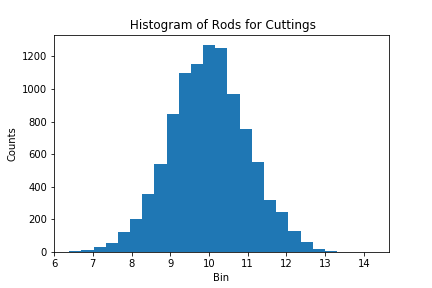
\includegraphics[width=0.7\linewidth,height=0.5\textheight]{Fig01}
\caption{1. Histogram Rods Variation}
\label{fig:Fig01}
\end{figure}


\end{frame}

\begin{frame}
\frametitle{9 Equipment}
\begin{equation}
\begin{minipage}{300pt}
 $\displaystyle f_{1} = NormalDistribution(0.5, 0.1)$  
\end{minipage}
\end{equation}
\begin{equation}
\begin{minipage}{300pt}
 $\displaystyle f{_1}(z) = \frac{5.0 \sqrt{2} e^{- 50.0 \left(z - 0.5\right)^{2}}}{\sqrt{\pi}}$  
\end{minipage}
\end{equation}
\begin{equation}
\begin{minipage}{300pt}
 $\displaystyle f{_2}(z) = \int_{z_{i}}^{z_{f}} f{_1}(z)\, dz$  
\end{minipage}
\end{equation}
\begin{equation}
\begin{minipage}{300pt}
 $\displaystyle Cut_{event} = random.normal(0.5, 0.1, 6880) =  \newline  [0.6953260727881961, 0.3332710414330152, \dots \\ 0.58874893292631] $  
\end{minipage}
\end{equation}

\end{frame}

\begin{frame}
\frametitle{10 Equipment Variable Histogram}
\noindent The histogram of (19) is shown in Figure 2.
\begin{figure}[H]
\centering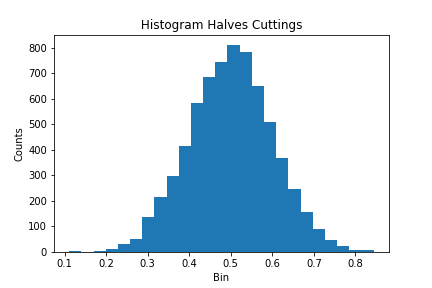
\includegraphics[width=1\linewidth,height=0.7\textheight]{Fig02}
\caption{2. Histogram of Cutter Variation}
\label{fig:Fig02}
\end{figure}


\end{frame}

\begin{frame}
\frametitle{11 Method}
\noindent Method 1\\ \ \\     From an end point the cutter is placed 5m away. The rod is placed against     that end point.\\ \ \\     Method 2 \\ \ \\     The cutter is located at the center of two end points. The rod is placed     between the end ponts. The end points are moved to hold the rod at the     center of the cutter. \\ \ \\     Question: Determine the formula for each and justify it.

\end{frame}

\begin{frame}
\frametitle{12 Method Variable}
\noindent Answers: \\ \ \\  1. The cutter with variation, i.e., $0.5 \pm .1$  is    multiplied by the perfect dimension of rod that is 10. Why perfect 10?    Then the answer is substracted from a rod with variation. The two answers    are the cut products. \\ \ \\    2. The rod with variation, i.e., $ 10 \pm 1$ is multiplied by the    cutter with variation, i.e., $0.5 \pm .1$. The answer is substracted from    the rod with variation. The two cuts are products. \\ 

\end{frame}

\begin{frame}
\frametitle{13 Method Histogram}
\noindent The histograms of Method 1 and 2 are shown in Figure 3.
\begin{figure}[H]
\centering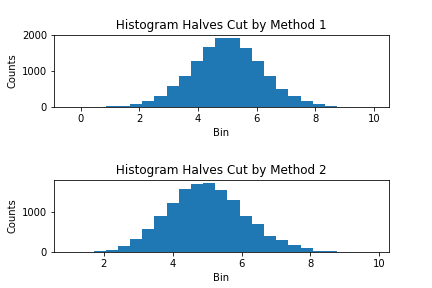
\includegraphics[width=1\linewidth,height=0.7\textheight]{Fig03}
\caption{3. Histogram of Cut Rods}
\label{fig:Fig03}
\end{figure}


\end{frame}

\begin{frame}
\frametitle{14 Method Yield}
\noindent Question: \\ \ \\    Assuming that the cut specification is $5 \pm .5$,    determine the number of good cut and the yield for each method \\ \ \\ 
\noindent Answer: \\ \ \\ 1. The number of good cut for method 1 is $4523 $ while for method 2 $4751 $ respectively. \\ \ \\ 
\noindent 2. The yield for method 1 is $32.8706 $\% while for method 2 is $34.5276 $\% respectively. Why is it method 2 has higher yield? \\ \ \\    \subsection{Operator} 

\end{frame}

\begin{frame}
\frametitle{15 Operator Handling}
\noindent Assume and operator makes the loading with error of $\mu = 0.4 $ and $\sigma = 0.1 $. \\ \ \\ \ The histograms with operator    handling for Method 1 and 2 are shown in Figure 4. \\ \ \\    The yield with operator's handling errors for method 1 is $32 $\% while for method 2 is $33 $\% respectively.

\end{frame}

\begin{frame}
\frametitle{16 Operator Handling Impact}
\begin{figure}[H]
\centering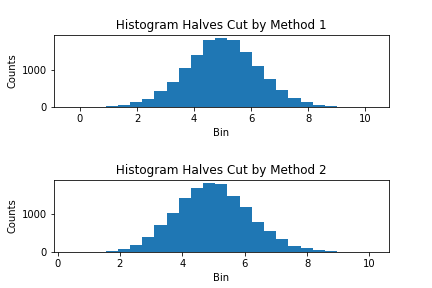
\includegraphics[width=1\linewidth,height=0.6\textheight]{Fig04}
\caption{4. Histogram of Cut Rods with    Operator's Handling}
\label{fig:Fig04}
\end{figure}


\end{frame}

\begin{frame}
\frametitle{17 Discussion on Sources of Variation}
\noindent $\bullet$Material mitigated by tighter tolerance with increased cost \\ \ \\     $\bullet$Machine mitigated by maintenance and continuous improvements \\ \ \\     $\bullet$Method generally difficult to observe and isolate and modelled,  \\ \ \\     $\bullet$Man mitigated by error proofing or Poka Yoke.

\end{frame}

\begin{frame}
\frametitle{18 Random Variable Models}
\noindent $\bullet$Consider a unit circle where an equilateral triangle is inscribed as     shown in Figure 5. \\ \ \\     $\bullet$ Suppose a random line is to be drawn across it,     determine the probability that the cord is less than the length of the     the side of equilateral triangle. \\ 

\end{frame}

\begin{frame}
\frametitle{19 Random Lines Across a Circle}
\begin{figure}[H]
\centering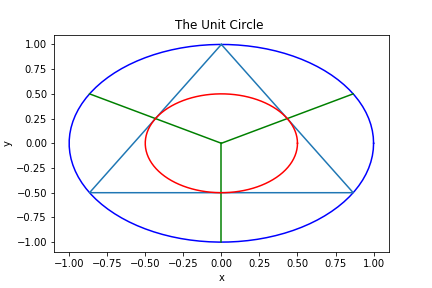
\includegraphics[width=1\linewidth,height=0.7\textheight]{Fig05}
\caption{5. Equilateral Triangle Inscribe in     Unit Circle}
\label{fig:Fig05}
\end{figure}


\end{frame}

\begin{frame}
\frametitle{20 Matter of Method}
\noindent There are a number of answer depending    on how the random lines are drawn. \\    1. The line drawn from any two points at the circumference, gives the    probability of $\frac{1}{3}$. \\    2. The line drawn perpendicular to radius from a any point along radius gives the    probability of $\frac{1}{2}$ \\    3. The line drawn tangent to any concentric circle gives the probabiity    $\frac{1}{4}$. \\    4. From the length of the cord i.e. $0$ to $2$, the probability is    $\frac{\sqrt{3}}{2}$. \\ \ \\    The question is that which of the four probability numbers make sense?    In all these methods, does rotation of line matters?

\end{frame}

\begin{frame}
\frametitle{21 Matter of Random Variables}
\noindent $\bullet$The random variable in matter of two points at the circumference is the    arc of the circle. \\ \ \\    $\bullet$The random variable for line drawn perpendiculare to the radius is the    distance of the point where line intersects with radius from the center of the circule.    \\ \ \\    $\bullet$The random variable for the line tangent to the concentric circle is the    area of the concentric circle. \\ \ \\    $\bullet$The random variable for the length of the cord is the cord itself. \\    -All the lines segmented by perimeter of the circle are cords. Why is it that    are the probabilities of the lines above are different from the last?

\end{frame}

\begin{frame}
\frametitle{22 Sample Problems}
\noindent Given a set of wirebonders bonding a particular producted, must all the set up     be identical exactly? \\ \ \\     Generally no however the ranges of parameters must be identical. It means     each machine is different and the parameters are used to nullify the     differences. \\ \ \\     The question is that what are the variables to be considered random?     These variables are not readily observable and measurable. These manifest     at region of ignorance where it is bounded by upper and lower control     limits of SPC charts

\end{frame}

\begin{frame}
\frametitle{23 Conclusion}
\noindent There are a number of innovation opportunities that may be derived. \\ \ \\     $\bullet$ Make the intermittent or not readily observable phenomenon     consistently observable \\ \ \\     $\bullet$ What is made consistently observable may not be readily measurable.     Therefore make it readily measurable. \\ \ \\     $\bullet$ The region of ignorance in SPC charts provides the leading clues     for such phenomenon.

\end{frame}

\begin{frame}
\frametitle{24 End of Presentation}
\noindent Maraming Salamat Po.

\end{frame}

\end{document}